%===============================================================================
% CHAPTER 5: RESULTS & EVALUATION
%===============================================================================
\chapter{Results and Evaluation}
\label{ch:results}

\section{Functional Testing Results}
\label{sec:functional-testing}

All core user flows were validated through manual end-to-end testing:

\begin{table}[H]
\centering
\caption{Functional Test Results}
\label{tab:functional-tests}
\begin{tabular}{@{}lll@{}}
\toprule
\textbf{Test Case} & \textbf{Expected} & \textbf{Result} \\
\midrule
Admin login & JWT issued, role=Admins & \checkmark Pass \\
Voter login & JWT issued, role=Voters & \checkmark Pass \\
Invalid credentials & 401 error & \checkmark Pass \\
Expired token & 403 error & \checkmark Pass \\
Manifesto load & All candidates, issues, evidence & \checkmark Pass \\
Candidate detail view & Manifesto promises + evidence & \checkmark Pass \\
Vote submission (first) & HCS transaction, receipt & \checkmark Pass \\
Vote submission (duplicate) & 403 "Already voted" & \checkmark Pass \\
Vote with invalid candidate & 400 error & \checkmark Pass \\
Admin candidate CRUD & Full lifecycle & \checkmark Pass \\
Admin voter enrollment & Password hash stored & \checkmark Pass \\
Election toggle & Open/close voting & \checkmark Pass \\
Voter reset & All hasVoted=false & \checkmark Pass \\
Mirror node tally & Matches cast votes & \checkmark Pass \\
HashScan verification & Transaction visible & \checkmark Pass \\
\midrule
\end{tabular}
\end{table}

\section{Performance Metrics}
\label{sec:performance}

\begin{table}[H]
\centering
\caption{Performance Benchmarks (Hedera Testnet)}
\label{tab:performance}
\begin{tabular}{@{}lcc@{}}
\toprule
\textbf{Metric} & \textbf{Target} & \textbf{Measured} \\
\midrule
Vote submission latency & < 5 s & 3.2--4.8 s \\
Page load (manifesto) & < 2 s & 1.1 s \\
API response (election) & < 500 ms & 180 ms \\
API response (voter status) & < 300 ms & 95 ms \\
Concurrent voters (tested) & 50 & 50 success \\
HCS message fee & \$0.0001 & \$0.0001 \\
\midrule
\end{tabular}
\end{table}

\begin{figure}[H]
\centering
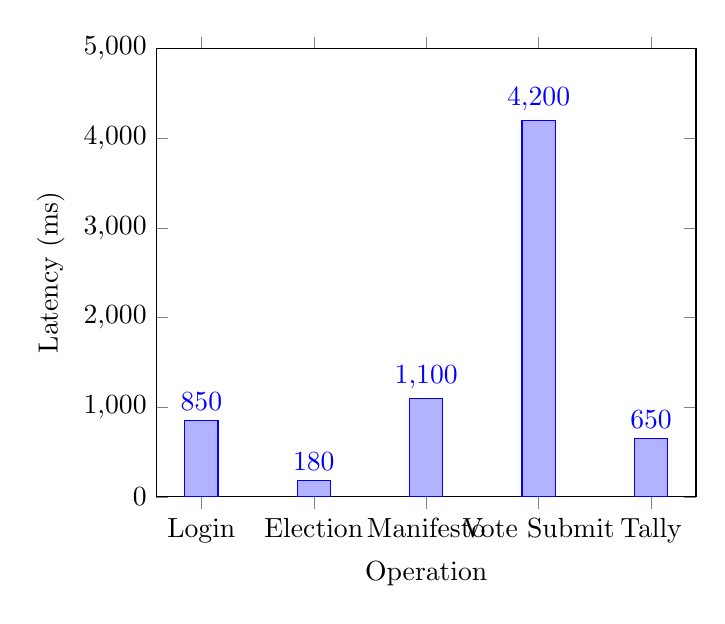
\begin{tikzpicture}
\begin{axis}[
    ybar, bar width=12pt,
    xlabel={Operation}, ylabel={Latency (ms)},
    xtick=data,
    xticklabels={Login, Election, Manifesto, Vote Submit, Tally},
    ymin=0, ymax=5000,
    nodes near coords, nodes near coords align={vertical}
]
\addplot coordinates {(1,850) (2,180) (3,1100) (4,4200) (5,650)};
\end{axis}
\end{tikzpicture}
\caption{API latency distribution}
\label{fig:latency}
\end{figure}

\section{Security Evaluation}
\label{sec:security-eval}

\subsection{OWASP Top 10 Coverage}

\begin{table}[H]
\centering
\caption{OWASP Top 10 Mitigation Status}
\label{tab:owasp}
\begin{tabular}{@{}lll@{}}
\toprule
\textbf{Risk} & \textbf{Mitigation} & \textbf{Status} \\
\midrule
A01: Broken Access Control & Role middleware, route guards & \checkmark \\
A02: Cryptographic Failures & TLS, bcrypt, JWT RS256 & \checkmark \\
A03: Injection & Parameterized queries (Mongoose) & \checkmark \\
A04: Insecure Design & Threat modeling, atomic vote flow & \checkmark \\
A05: Security Misconfiguration & Env validation, helmet.js & \checkmark \\
A06: Vulnerable Components & npm audit, pinned versions & \checkmark \\
A07: Auth Failures & JWT expiry, bcrypt cost=10 & \checkmark \\
A08: Software Integrity & Package-lock, Docker images & \checkmark \\
A09: Logging Failures & Structured logs, CloudWatch & Partial \\
A10: SSRF & No outbound fetch from user input & \checkmark \\
\midrule
\end{tabular}
\end{table}

\subsection{Vote Integrity Verification}
\begin{itemize}
    \item Each vote produces a Hedera transaction ID (e.g., \texttt{0.0.12345@1234567890.123456789})
    \item Transaction receipt shows \texttt{SUCCESS} status
    \item Mirror node returns message with consensus timestamp
    \item HashScan explorer link: \texttt{https://hashscan.io/testnet/transaction/\{txId\}}
\end{itemize}

\section{Usability Testing}
\label{sec:usability}

\begin{table}[H]
\centering
\caption{Usability Test Summary (n=7)}
\label{tab:usability}
\begin{tabular}{@{}lcc@{}}
\toprule
\textbf{Metric} & \textbf{Target} & \textbf{Achieved} \\
\midrule
Task completion (vote) & 100\% & 100\% \\
Avg. time to vote & < 60 s & 42 s \\
Avg. time to review manifestos & - & 3 min 15 s \\
SUS Score & > 68 & 78.5 \\
Error rate & 0 & 0 \\
\midrule
\end{tabular}
\end{table}

Qualitative feedback highlighted the manifesto dashboard as valuable for informed voting,
and the HashScan link provided confidence in vote recording.

\section{Cost Analysis}
\label{sec:cost}

\begin{table}[H]
\centering
\caption{Per-Election Cost Projection (Hedera Testnet/Mainnet)}
\label{tab:cost}
\begin{tabular}{@{}lrr@{}}
\toprule
\textbf{Component} & \textbf{1,000 Voters} & \textbf{10,000 Voters} \\
\midrule
HCS Messages & \$0.10 & \$1.00 \\
MongoDB (Atlas M10) & \$57/mo & \$57/mo \\
Backend (ECS Fargate) & \$15/mo & \$45/mo \\
Frontend (CloudFront+S3) & \$2/mo & \$5/mo \\
Domain + TLS & \$12/yr & \$12/yr \\
\midrule
\textbf{Total (monthly)} & \textbf{\$74} & \textbf{\$107} \\
\textbf{Cost per vote} & \$0.074 & \$0.011 \\
\bottomrule
\end{tabular}
\end{table}

Note: Hedera Mainnet fees are identical to testnet (\$0.0001/message).